\section{预备知识及技能}
\subsection{RISC-V和LoongArch指令集介绍}
\textbf{1、RISC-V}

RISC-V(发音为“risk-five”)是一个基于精简指令集(RISC)原则的开源指令集架构(ISA),简易解释为开源软体运动相对应的一种“开源硬体”。该项目2010年始于加州大学柏克莱分校,但许多贡献者是该大学以外的志愿者和行业工作者。\\
与大多数指令集相比,RISC-V指令集可以自由地用于任何目的,允许任何人设计、制造和销售RISC-V芯片和软件而不必支付给任何公司专利费。虽然这不是第一个开源指令集,但它具有重要意义,因为其设计使其适用于现代计算设备(如仓库规模云计算机、高端移动电话和微小嵌入式系统)。设计者考虑到了这些用途中的性能与功率效率。该指令集还具有众多支持的软件,这解决了新指令集通常的弱点。\\
RISC-V指令集的设计考虑了小型、快速、低功耗的现实情况来实做,但并没有对特定的微架构做过度的设计。
新出现的RISC-V的核心目标是灵活适应未来的AIoT场景,保证基本功能,提供可配置的扩展功能。其开源特征使得学生都可以方便地设计一个RISC-V CPU。\\
写面向RISC-V的OS的代价仅仅是你了解RISC-V的Supevisor特权模式,知道OS在Supevisor特权模式下的控制能力。\\
\textbf{2、 LoongArch}

LoongArch是RISC中的一个具体实现。2020年,龙芯中科基于二十年的CPU研制和生态建设积累推出了龙架构(LoongArch™),包括基础架构部分和向量指令、虚拟化、二进制翻译等扩展部分,近2000条指令。

龙架构具有较好的自主性、先进性与兼容性。

龙架构从整个架构的顶层规划,到各部分的功能定义,再到细节上每条指令的编码、名称、含义,在架构上进行自主重新设计,具有充分的自主性。

龙架构摒弃了传统指令系统中部分不适应当前软硬件设计技术发展趋势的陈旧内容,吸纳了近年来指令系统设计领域诸多先进的技术发展成果。同原有兼容指令系统相比,不仅在硬件方面更易于高性能低功耗设计,而且在软件方面更易于编译优化和操作系统、虚拟机的开发。

龙架构在设计时充分考虑兼容生态需求,融合了各国际主流指令系统的主要功能特性,同时依托龙芯团队在二进制翻译方面十余年的技术积累创新,能够实现多种国际主流指令系统的高效二进制翻译。龙芯中科从 2020 年起新研的 CPU 均支持LoongArch™。

龙架构已得到国际开源软件界广泛认可与支持,正成为与X86/ARM并列的顶层开源生态系统。已向GNU组织申请到ELF Machine编号(258号),并获得Linux、Binutils、GDB、.NET、GCC、LLVM、Go、Chromium/V8、Mozilla / SpiderMonkey、Javascript、FFmpeg、libyuv、libvpx、OpenH264、SRS等音视频类软件社区、UEFI(UEFI规范、ACPI规范)以及国内龙蜥开源社区、欧拉openEuler开源社区的支持。

指令系统是软件生态的起点,只有从指令系统的根源上实现自主,才能打破软件生态发展受制于人的锁链。龙架构的推出,是龙芯中科长期坚持自主研发理念的重要成果体现,是全面转向生态建设历史关头的重大技术跨越。

\subsection{Rust语言及其主要特性}
Rust是由Mozilla主导开发的通用、编译型编程语言。设计准则为“安全、并发、实用”,支持函数式、并发式、过程式以及面向对象的程序设计风格。

Rust语言原本是Mozilla员工Graydon Hoare的个人项目,而Mozilla于2009年开始赞助这个项目,并且在2010年首次公开。也在同一年,其编译器原始码开始由原本的OCaml语言转移到用Rust语言,进行自我编译工作,称做“rustc”,并于2011年实际完成。这个可自我编译的编译器在架构上采用了LLVM做为它的后端。

第一个有版本号的Rust编译器于2012年1月发布。Rust1.0是第一个稳定版本,于2015年5月15日发布。

Rust在完全公开的情况下开发,并且相当欢迎社区的反馈。在1.0稳定版之前,语言设计也因为透过撰写Servo网页浏览器排版引擎和rustc编译器本身,而有进一步的改善。它虽然由Mozilla资助,但其实是一个共有项目,有很大部分的代碼是来自于社区的贡献者。

\textbf{1.所有权}

所有权是Rust的核心,也是其更有趣和独特的功能之一。“所有权”是指允许哪部分的代码修改内存。让我们从查看一些C++代码开始:
\begin{lstlisting}[language={Rust}, label={code:forktest},
	caption={forktest.rs}]
	int *dangling(void)
	{
		int i = 1234;
		return &i;
	}
	
	int add_one(void)
	{
		int *num = dangling();
		return *num + 1;
	}
\end{lstlisting}

dangling函数在栈上分配了一个整型,然后保存给一个变量i,最后返回了这个变量i的引用。这里有一个问题:当函数返回时栈内存变成失效。意味着在函数add\_one第二行,指针num指向了垃圾值,我们将无法得到想要的结果。虽然这个一个简单的例子,但是在C++的代码里会经常发生。当堆上的内存使用malloc(或new)分配,然后使用free(或delete)释放时,会出现类似的问题,但是您的代码会尝试使用指向该内存的指针执行某些操作。 更现代的C++使用RAII和构造函数/析构函数,但它们无法完全避免“悬空指针”。 这个问题被称为“悬空指针”,并且不可能编写出现“悬空指针”的Rust代码。 我们试试吧:
\begin{lstlisting}[language={Rust}, label={code:forktest},
	caption={forktest.rs}]
	fn dangling() -> &int {
		let i = 1234;
		return &i;
	}
	
	fn add_one() -> int {
		let num = dangling();
		return *num + 1;
	}
\end{lstlisting}

当你尝试编译这个程序时,你会得到一个有趣和非常长的错误信息:
\begin{lstlisting}[language={Rust}, label={code:forktest},
	caption={forktest.rs}]
	temp.rs:3:11: 3:13 error: borrowed value does not live long enough
	temp.rs:3     return &i;
	
	temp.rs:1:22: 4:1 note: borrowed pointer must be valid for the anonymous lifetime #1 defined on the block at 1:22...
	temp.rs:1 fn dangling() -> &int {
		temp.rs:2     let i = 1234;
		temp.rs:3     return &i;
		temp.rs:4 }
	
	temp.rs:1:22: 4:1 note: ...but borrowed value is only valid for the block at 1:22
	temp.rs:1 fn dangling() -> &int {      
		temp.rs:2     let i = 1234;            
		temp.rs:3     return &i;               
		temp.rs:4  }                            
	error: aborting due to previous error
\end{lstlisting}

为了完全理解这个错误信息,我们需要谈谈“拥有”某些东西意味着什么。 所以现在,让我们接受Rust不允许我们用悬空指针编写代码,一旦我们理解了所有权,我们就会回来看这块代码。

让我们先放下编程一会儿,先聊聊书籍。 我喜欢读实体书,有时候我真的很喜欢一本书,并告诉我的朋友他们应该阅读它。 当我读我的书时,我拥有它:这本书是我所拥有的。 当我把书借给别人一段时间,他们向我“借用”这本书。 当你借用一本书时,在特定的一段时间它是属于你的,然后你把它还给我,我又拥有它了。 对吗?

这个概念也直接应用于Rust代码:一些代码“拥有”一个指向内存的特定指针。 它是该指针的唯一所有者。 它还可以暂时将该内存借给其他代码:代码“借用”它。 借用它一段时间,称为“生命周期”。

这是关于所有权的所有。 那似乎并不那么难,对吧? 让我们回到那条错误信息:error: borrowed value does not live long enough。 我们试图使用Rust的借用指针&,借出一个特定的变量i。 但Rust知道函数返回后该变量无效,因此它告诉我们:
\begin{lstlisting}[language={Rust}, label={code:forktest},
	caption={forktest.rs}]
	borrowed pointer must be valid for the anonymous lifetime #1
	
	... but borrowed value is only valid for the block。
\end{lstlisting}

这是栈内存的一个很好的例子,但堆内存呢? Rust有第二种指针,一个'唯一'指针,你可以用$\sim$创建。 看看这个:
\begin{lstlisting}[language={Rust}, label={code:forktest},
	caption={forktest.rs}]
	fn dangling() -> ~int {
		let i = ~1234;
		return i;
	}
	
	fn add_one() -> int {
		let num = dangling();
		return *num + 1;
	}
\end{lstlisting}

此代码将成功编译。 请注意,我们使用指针指向该值而不是将1234分配给栈:$\sim$1234。 你可以大致比较这两行:
\begin{lstlisting}[language={Rust}, label={code:forktest},
	caption={forktest.rs}]
	// rust
	let i = ~1234;
	// C++
	int *i = new int;
	*i = 1234;
\end{lstlisting}

Rust能够推断出类型的大小,然后分配正确的内存大小并将其设置为您要求的值。 这意味着无法分配未初始化的内存:Rust没有null的概念。万岁! Rust和C++之间还有另外一个区别:Rust编译器还计算了i的生命周期,然后在它无效后插入相应的free调用,就像C++中的析构函数一样。 您可以获得手动分配堆内存的所有好处,而无需自己完成所有工作。 此外,所有这些检查都是在编译时完成的,因此没有运行时开销。 如果你编写了正确的C++代码,你将编写出与C++代码基本上相同的Rust代码。而且由于编译器的帮忙,编写错误的代码版本是不可能的。
你已经看到了一种情况,所有权和生命周期有利于防止在不太严格的语言中通常会出现的危险代码。现在让我们谈谈另一种情况:并发。

\textbf{2.并发:}

并发是当前软件世界中一个令人难以置信的热门话题。 对于计算机科学家来说,它一直是一个有趣的研究领域,但随着互联网的使用爆炸式增长,人们正在寻求改善给定的服务可以处理的用户数量。 并发是实现这一目标的一种方式。 但并发代码有一个很大的缺点:它很难推理,因为它是非确定性的。 编写好的并发代码有几种不同的方法,但让我们来谈谈Rust的所有权和生命周期的概念如何帮助实现正确并且并发的代码。

首先,让我们回顾一下Rust中的简单并发示例。 Rust允许你启动task,这是轻量级的“绿色”线程。 这些任务没有任何共享内存,因此,我们使用“通道”在task之间进行通信。 像这样:
\begin{lstlisting}[language={Rust}, label={code:forktest},
	caption={forktest.rs}]
	fn main() {
		let numbers = [1,2,3];
		
		let (port, chan)  = Chan::new();
		chan.send(numbers);
		
		do spawn {
			let numbers = port.recv();
			println!("{:d}", numbers[0]);
		}
	}
\end{lstlisting}

在这个例子中,我们创建了一个数字的vector。 然后我们创建一个新的Chan,这是Rust实现通道的包名。 这将返回通道的两个不同端:通道(channel)和端口(port)。 您将数据发送到通道端(channel),它从端口端(port)读出。 spawn函数可以启动一个task。 正如你在代码中看到的那样,我们在task中调用port.recv(),我们在外面调用chan.send(),传入vector。 然后打印vector的第一个元素。

这样做是因为Rust在通过channel发送时copy了vector。 这样,如果它是可变的,就不会有竞争条件。 但是,如果我们正在启动很多task,或者我们的数据非常庞大,那么为每个任务都copy副本会使我们的内存使用量膨胀而没有任何实际好处。

引入Arc。 Arc代表“原子引用计数”,它是一种在多个task之间共享不可变数据的方法。 这是一些代码:
\begin{lstlisting}[language={Rust}, label={code:forktest},
	caption={forktest.rs}]
	extern mod extra;
	use extra::arc::Arc;
	
	fn main() {
		let numbers = [1,2,3];
		
		let numbers_arc = Arc::new(numbers);
		
		for num in range(0, 3) {
			let (port, chan)  = Chan::new();
			chan.send(numbers_arc.clone());
			
			do spawn {
				let local_arc = port.recv();
				let task_numbers = local_arc.get();
				println!("{:d}", task_numbers[num]);
			}
		}
	}
\end{lstlisting}

这与我们之前的代码非常相似,除了现在我们循环三次,启动三个task,并在它们之间发送一个Arc。 Arc :: new创建一个新的Arc,.clone()返回Arc的新的引用,而.get()从Arc中获取该值。 因此,我们为每个task创建一个新的引用,将该引用发送到通道,然后使用引用打印出一个数字。 现在我们不copy vector。

Arcs非常适合不可变数据,但可变数据呢? 共享可变状态是并发程序的祸根。 您可以使用互斥锁(mutex)来保护共享的可变状态,但是如果您忘记获取互斥锁(mutex),则可能会发生错误。

Rust为共享可变状态提供了一个工具:RWArc。 Arc的这个变种允许Arc的内容发生变异。 看看这个:
\begin{lstlisting}[language={Rust}, label={code:forktest},
	caption={forktest.rs}]
	extern mod extra;
	use extra::arc::RWArc;
	
	fn main() {
		let numbers = [1,2,3];
		
		let numbers_arc = RWArc::new(numbers);
		
		for num in range(0, 3) {
			let (port, chan)  = Chan::new();
			chan.send(numbers_arc.clone());
			
			do spawn {
				let local_arc = port.recv();
				
				local_arc.write(|nums| {
					nums[num] += 1
				});
				
				local_arc.read(|nums| {
					println!("{:d}", nums[num]);
				})
			}
		}
	}
\end{lstlisting}

我们现在使用RWArc包来获取读/写Arc。 RWArc的API与Arc略有不同:读和写允许您读取和写入数据。 它们都将闭包作为参数,并且在写入的情况下,RWArc将获取互斥锁,然后将数据传递给此闭包。 闭包完成后,互斥锁被释放。

你可以看到在不记得获取锁的情况下是不可能改变状态的。 我们获得了共享可变状态的便利,同时保持不允许共享可变状态的安全性。

但是我们不能同时允许和禁止可变状态。 是什么赋予了这种能力的?

\textbf{3.unsafe:}

因此,Rust语言不允许共享可变状态,但我刚刚向您展示了一些允许共享可变状态的代码。 这怎么可能? 答案:unsafe。

你看,虽然Rust编译器非常聪明,并且可以避免你通常犯的错误,但它不是人工智能。 因为我们比编译器更聪明,有时候,我们需要克服这种安全行为。 为此,Rust有一个unsafe关键字。 在一个unsafe的代码块里,Rust关闭了许多安全检查。 如果您的程序出现问题,您只需要审核您在不安全范围内所做的事情,而不是整个程序。

如果Rust的主要目标之一是安全,为什么要关闭安全?
嗯,实际上只有三个主要原因:与外部代码连接,例如将FFI写入C库,性能(在某些情况下),以及围绕通常不安全的操作提供安全抽象。 我们的Arcs是最后一个目的的一个例子。 我们可以安全地分发对Arc的多个引用,因为我们确信数据是不可变的,因此可以安全地共享。 我们可以分发对RWArc的多个引用,因为我们知道我们已经将数据包装在互斥锁中,因此可以安全地共享。 但Rust编译器无法知道我们已经做出了这些选择,所以在Arcs的实现中,我们使用不安全的块来做(通常)危险的事情。 但是我们暴露了一个安全的接口,这意味着Arcs不可能被错误地使用。

这就是Rust的类型系统如何让你不会犯一些使并发编程变得困难的错误,同时也能获得像C++等语言一样的效率。

我希望这个对Rust的尝试能让您了解Rust是否适合您。 如果这是真的,我建议您查看完整的教程,以便对Rust的语法和概念进行全面,深入的探索。
\subsection{如何查资料}
\textbf{1、查手册}

\textbf{程序自带的文档}
(1) README 和 INSTALL

很多程序在编译或者安装过程中都会自带一个README和INSTALL文件, 不要漏掉, 否则可能会有重要的信息遗漏并导致某些严重问题。

其中, 如果INSTALL文件被单独呈现, 则其往往是解释软件的安装方式的, 有的软件有很特殊的安装要求, 如执行脚本的位置必须是在文件夹内或者文件夹外, 如果漏掉可能导致软件完全运行不起来。

README一般介绍软件的使用方式, 文档获取位置和帮助信息, 有时候也介绍安装方法。

例如, 你在NPUcore的源代码文件夹中可以找到README:
\begin{figure}[htb]
	\centering
	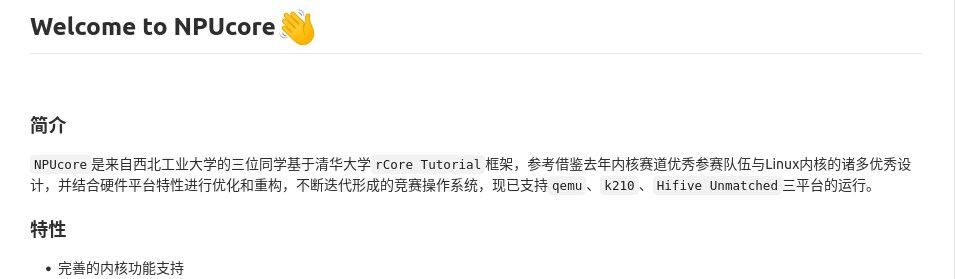
\includegraphics[width=\textwidth]{figures/02-01-readme.png}
	\caption{
		readme
	}
	\label{fig:readme}
\end{figure}
(2) help参数
绝大多数程序会自带一个help选项, 甚至不加任何参数。 例如, man命令的help参数:

\begin{lstlisting}[language={Rust}, label={code:forktest},
	caption={forktest.rs}]
	whatis --help
\end{lstlisting}

会打印出:
\begin{figure}[htb]
	\centering
	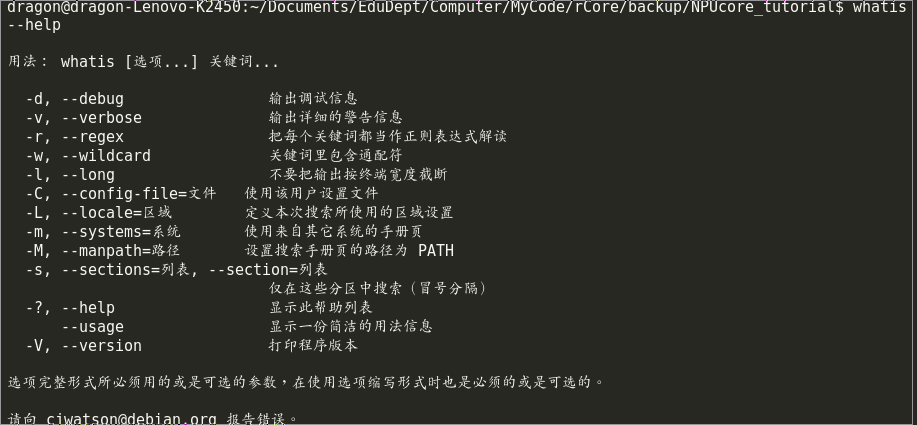
\includegraphics[width=\textwidth]{figures/02-01-help.png}
	\caption{
		help
	}
	\label{fig:help}
\end{figure}
那么, 如果你直接在终端中敲入help并回车, 会发生什么呢(假设你使用的是bash)?请自己试一下.

此外, 帮助文档的提供软件自身往往也会有自己的帮助文档, 显然自产自销是最合适的。

所以, 你不妨试一下man man, 或者进入man后有没有能看到的某些man自己的帮助文档(仔细找, 我这么说就一定有)。

之后的任何帮助套件也可以“自己帮助自己”, 所以文献中不再赘述。

(3) TAB补全

在Bash中,TAB补全是一种非常有用的功能,它可以让用户更快捷、更准确地输入命令和文件路径。在终端输入命令或文件路径时,如果按下TAB键,Bash会尝试自动补全输入的内容。

下面是关于Bash中TAB补全常见类型(如果没有特别说明, 则Bash会列出这些选项供选择):
1)命令补全:输入一个命令的前几个字母时,补全该命令的名称。如果有多个以该字符串开头的命令,
2)文件路径补全:输入一个文件或目录的路径时,补全路径中的文件或目录名称。如果有多个符合条件的文件或目录,
3)变量名补全:输入一个变量名时,补全该变量的名称。如果有多个符合条件的变量名,
4)命令参数补全:输入命令的参数时,补全该命令所支持的参数选项。如果有多个符合条件的参数选项,
5)目录补全:在输入路径时,如果您只知道路径中的某些部分,可以使用通配符进行补全。例如,输入"/u/lo*",按下TAB键可以自动补全为"/usr/local"。

总之,bash中的TAB补全是一种非常方便的功能,可以让用户更快速地输入命令和路径,并且减少输入错误的可能性。

此外, TAB补全需要程序自身和终端的支持, 有时候甚至需要单独配置, (例如rust的工具链就需要自行配置对应的shell补全选项)

\textbf{man}

在Linux操作系统中,man命令是一个非常重要的命令,它可以帮助用户查看Linux系统中各种命令的手册。

使用man只需要在终端中输入"man"加上要查看的命令名称,然后按下回车键即可。例如:

\begin{lstlisting}[language={Rust}, label={code:forktest},
	caption={forktest.rs}]
	man help
\end{lstlisting}

man命令将会显示出该命令的手册页,可以使用键盘上的箭头键进行滚动,并且可以使用“/”加上关键字进行查找。

在手册页中,可以查看该命令的使用方法、参数选项、示例以及其他相关信息。 man软件的本身的帮助信息可以在软件中按“h”查看。

当不再需要查看手册页时,可以按下“q”键退出man命令。

\textbf{完整手册}
多数成体系的大型软件系统会有自己对应的文档, 一般称为手册. 具体来说, 这种文档会出现在官方网站的Documentation环节, 且往往有在线或者线下PDF两种版本。

我们以GNU GCC为例, 在https://gcc.gnu.org/中, 浏览器搜索(一般快捷键是Ctrl-F)Documentation, 下方的Manual就是手册。点进去会有各种格式的手册。

有的成熟的软件或者语言会提供Tutorial 和 Reference Manual, 后者倾向于列举所有的性质, 前者则是为入门初学者提供的简单的教程。

一般而言, 绝大多数的软件是自身具有自己的手册的, 但部分软件的手册是集合型的, 或者本身就是其manpage的集合。

一个典型的例子是coreutils, 其中包括了cut, head, tail等简单工具;另一个是binutils, 包括各种GCC的常用工具。这时候需要自行查询其手册的所在之处。

\textbf{教材}

很多的软件都有自己的教材, 且层次从入门到精通都有, 如果你有需要, 可以找买一本合适的书从中学习。 一般教材会比官方手册更详细, 并提供作者自己的思考。

\textbf{TLDR}

TLDR是“Too long, don't read.”的缩写,
如果要最快获得某个命令的简单使用方法, tldr是一个不错的来源。例如我们输入

\begin{lstlisting}[language={Rust}, label={code:forktest},
	caption={forktest.rs}]
	$ tldr man
	
	Format and display manual pages.More information: https://www.man7.org/linux/man-pages/man1/man.1.html.
	
	- Display the man page for a command:
	man {{command}}
	
	- Display the man page for a command from section 7:
	man {{7}} {{command}}
	
	- List all available sections for a command:
	man -f {{command}}
	
	- Display the path searched for manpages:
	man --path
	
	- Display the location of a manpage rather than the manpage itself:
	man -w {{command}}
	
	- Display the man page using a specific locale:
	man {{command}} --locale={{locale}}
	
	- Search for manpages containing a search string:
	man -k "{{search_string}}"
\end{lstlisting}

\textbf{info}

注意, info是用某个目录作为中心数据库的, 所以完全可能存在在一个软件中可以阅读但在另一个软件中读不了的情况。

info中有大量长篇的完整文档, 一般就是上述完整手册。 一般各种IDE本身也会自带Info的阅读器。 只是info有自己的搜索, 历史记录等功能(有的功能是配合IDE使用的), 这里不再赘述。

此外, GNU套件几乎所有的工具都有info文档。所谓的GNU套件PDF文档就是用info相关的一个软件texinfo写的。

我们以gdb为例展示其内容。 终端输入“info gdb”可以得到:

\begin{figure}[htb]
	\centering
	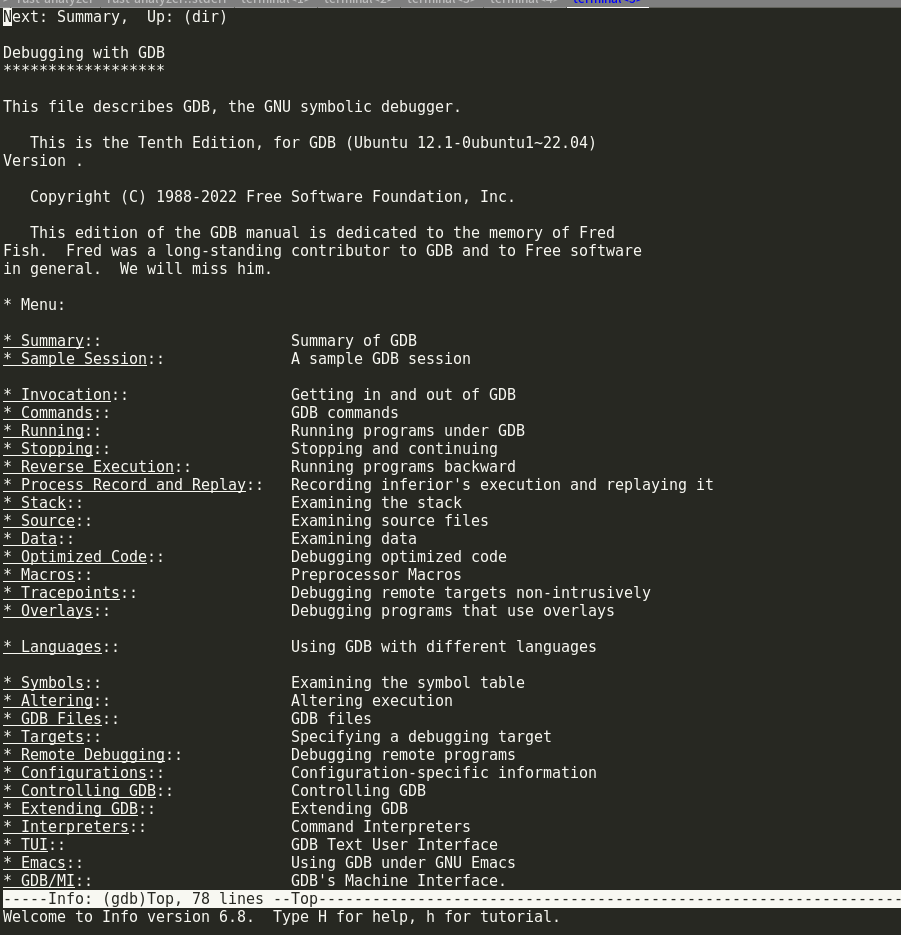
\includegraphics[width=\textwidth]{figures/02-01-info.png}
	\caption{
		info
	}
	\label{fig:info}
\end{figure}

另外, info文档的安装方法如下:

对于软件自带文档,一般可以:

\begin{lstlisting}[language={Rust}, label={code:forktest},
	caption={info}]
	sudo apt-get install gdb-doc
	有时候需要去网站上搜索并下载, 就会需要:
	whereis info # 获得info的安装目录
	# 注意:有时候下载到的是一个info.tar.gz, 这时候需要自行解压, 
	# 但是如果是info.gz,则可以直接跳过这一步, 因为gz一般是自动解压的。
	# 另外,有时候文档是以texi后缀名出现的
	tar xf <infofilepath> <tmp_path>
	sudo install-info bison.info <one_of_the_info_paths>/dir
\end{lstlisting}

\textbf{自动补全与文档显示插件}

多数的IDE有自己的文档现实和自动补全插件, 可以在光标悬停在某个符号一段时间后自动显示特定的文档。

很多IDE还会集成之前的所说的这些文档查询方式, 从而在内部查询所有的文献。

请自行搜索自己的编辑器和IDE的文档寻找配置方式。

\textbf{搜索引擎}

如果你遇到什么工具你无法使用或者不会用, 可以尝试通过搜索引擎寻找替代品, 在线版或者其他能让你用上的方法(比如能够代理你请求的某些接口,软件和网站)。

\textbf{论坛}

论坛往往是最后一步, 一般来说很少出现别人没有发现过而自己发现的问题, 毕竟计算机工业确实过于发达了. 但是, 在stackoverflow和其他论坛上提问仍然有可能可以获得比较好的效果。

如果人家恰好碰到过或者有兴趣帮你解决问题的话是再幸运不过的事, 不过在此之前, 请先不要往下看, 尝试通过之前几步查找可能技术论坛以便解决问题。

然后这是一份作者根据自己回忆写的常见的论坛, 你可以试着在上面发帖. 此外, 一般使用量大的项目都有自己的论坛, 你也可以自行查找。







